%% ============================================================
%% Breaking the Bubble? — REVISED DRAFT v4 (July 2026)
%%
%% CITATION SETUP (this is what fixes the broken references):
%%  * The sn-jnl class loads natbib ITSELF when given a reference-style
%%    option. Without an option, \citep/\citet are undefined — that is
%%    the error you saw. Here we use [pdflatex,sn-basic]: Springer
%%    Nature basic author-year style, natbib-compatible.
%%    Do NOT add \usepackage{natbib} on top; the class handles it.
%%  * \bibliography{sn-bibliography,new_references} at the end: replace
%%    "sn-bibliography" with the exact name of the .bib file in your
%%    Overleaf file tree (without extension). "new_references" is the
%%    companion file shipped with this draft; upload it next to main.tex.
%%
%% CITATION AUDIT (2026-07-13): all 73 cited keys verified — 59 are in
%% the compiled paper's reference list (incl. Barberá, Ekström,
%% Holguín-Veras, Søgaard, whose accents broke the earlier check);
%% 14 are supplied in new_references.bib. Four of those (glickman2024human,
%% lorenz2011social, becker2017network, bail2018exposure) may already be
%% in your Overleaf .bib under other keys — if so, either rename the keys
%% in this file or delete the duplicates from new_references.bib.
%% The unverifiable "Fu et al. 2023" citation was REMOVED from Methods
%% (TODO comment left in place).
%%
%% FIGURES: repository snapshot 2026-07-10 (branch
%% claude/disasterai-results-validation-i76ple). Upload the repo PNGs to
%% Overleaf, replacing older copies of the same names. Fig. 1 is TikZ
%% (compiles in-document). comparison_configs.png comes from the
%% comparison workflow (tools/compare_configs.py).
%%
%% [TO RE-RUN] flags remain for the cognitive-gap and factor sweeps.
%% ============================================================

\documentclass[pdflatex,sn-basic]{sn-jnl}

\usepackage{graphicx}
\usepackage{multirow}
\usepackage{amsmath,amssymb,amsfonts}
\usepackage{amsthm}
\usepackage{booktabs}
\usepackage{tikz}
\usetikzlibrary{arrows.meta,positioning,calc}

\begin{document}

\title[Breaking the Bubble?]{Breaking the Bubble? How Belief-Aligned AI Reshapes Collective Opinions and Decisions in Urgent Decisions}

\author*[1,2]{\fnm{Tina} \sur{Comes}}\email{t.comes@tudelft.nl}

\affil*[1]{\orgdiv{Faculty of Technology, Policy \& Management}, \orgname{TU Delft}, \orgaddress{\city{Delft}, \country{The Netherlands}}}
\affil[2]{\orgdiv{Institute for the Protection of Terrestrial Infrastructures}, \orgname{DLR}, \orgaddress{\city{Sankt Augustin}, \country{Germany}}}

\abstract{In an increasingly fragmented and complex world, AI promises to break echo chambers by giving everyone access to information. Yet information that contradicts beliefs risks being rejected. Therefore, AI trained on human feedback drifts towards sycophancy: confirming what its users already believe. The impact of AI has so far been primarily studied for individual situation awareness or decisions, yet echo chambers form in networks. To address this gap, this paper analyses how far an AI should align with human beliefs to be accepted and break social echo chambers, and how this impacts belief correctness and the quality of decisions. 

The problem of AI alignment is most acute in disasters, where high-stakes decisions under time pressure leave little room for verification, and where disrupted networks and local focus amplify fragmentation and misallocation of resources. We use an agent-based model of disaster response in which individuals contact peers or consult an AI, update their beliefs, and act on them by sending assistance. The AI has an alignment parameter $\alpha$ that varies it from sending perfect ground truth to fully confirming human beliefs. 

We report four findings. First, interaction structure decides on influence of AI: a confirming AI deepens social echo chambers only if information access follows social ties, feeding each community its own shared beliefs. Second, a fully truthful AI creates echo chambers of its own, converging the beliefs of the most AI-reliant users. Third, intermediate alignment ($\alpha* \approx$ 0.4–0.6) minimises social and AI-induced echo chambers while sustaining relief performance. Fourth, rising alignment concentrates harm on those who are remote from the disaster, who lose situational awareness and withdraw from the response; even highly connected network positions offer no protection. By taking belief-aligned AI from interaction of individuals with one AI to people as social beings interacting in communities, these findings shift the questions of alignment and sycophancy to a property of the sociotechnical system.}

%We humans increasingly delegate information collection, analysis and interpretation to AI systems. The promise of AI is to deliver data-driven support that helps overcome human cognitive biases and echo chambers. Yet many of the most recent AI systems are trained on human feedback and thereby become sycophantic: they tend to return what confirms a user's beliefs. Research on human-centred AI has begun to analyse how such belief-aligned AI affects individual judgement, but humans are social beings whose opinions form in communities and networks. What is missing is an understanding of how belief-aligned AI reshapes the information processing, beliefs and decisions within human communities. This paper views humans as social beings and puts their adaptive behaviour at the centre. An agent-based model simulates networked communities where individuals interact with each other or an AI to observe, learn and decide. An alignment parameter tunes theAI's reports between reporting ground truth and confirming an individuals beliefs. Human agents with exploratory or exploitative strategies select information sources through reinforcement learning and revise their beliefs through Bayesian updating. To understand the role of community structure,  we compare a configuration in which information access follows a spatially embedded social network and agent mobility with a control, in which any agent can consult any other. Three findings emerge. First, the organisation of the community decides the direction of AI influence: a belief-confirming AI deepens echo chambers only where information access follows social ties, because it recycles each community's consensus back into thecommunity. Second, networked communities have a bounded window of tolerable alignment: intermediate alignment ($\alpha^* \approx$ 0.4--0.6) minimises social and AI-induced echo chambers, outperforming a fully truthful AI as well as a fully confirming one, and coincides with the highest alignment at which echo chambers still dissolve within the response horizon. Third, the community's own learning loop buffers the operational damage of a confirming AI, so that relief performance degrades gradually where the control collapses; yet the residual harm is unequal and silent. As alignment rises, communities far from the disaster lose situational awareness fastest and progressively withdraw from the relief effort, while position in the social network offers no protection.How a belief-aligned AI harms a community therefore depends on how that community organises its information flows. Where anyone can consult anyone, sycophancy degrades collective decisions openly; in networked communities, decisions degrade only gradually while beliefs converge into an insularity that no longer recovers and whose burden falls on those furthest from the events, a failure that operational monitoring alone would miss. The degree of belief alignment of an AI and the structure of the community that adopts it must therefore be designed and monitored together.}

\keywords{Sycophancy, AI Alignment, Echo Chamber, Filter Bubble, Opinion Dynamics, Human--AI Interaction, Agent-Based Modelling, Disaster Response}

\maketitle

\section{Introduction}\label{sec:intro}
Societies are fragmenting into segregated information spaces. Online and offline echo chambers form, or information environments in which pre-existing beliefs and opinions are reinforced while exposure to diverse or contradictory perspectives is limited \citep{mahmoudi2024echo}. These echo chambers are associated with polarisation and the erosion of shared factual ground \citep{jeon2024, cinelli2021echo, bail2018exposure, baumann2020modeling}. 

Into this landscape, artificial intelligence (AI) arrives. Especially generative AI, via Large Language Models and chatbots promise to help humans interpret complex and highly uncertain information. Thus far, however, the use of LLMs so far is far from pervasive, and there are distinct groups who use (or not) LLMs \cite{angrisani2026gaps}, risking further amplification of polarisation. Yet, as we humans increasingly delegate the collection, analysis and interpretation of information to AI systems \citep{klingbeil2024}, the promise of AI is that these systems could give everyone access to accurate and tailored information beyond their own circles, correcting the biases and bridging the divides that human information
sharing produces \citep{jeon2024}. 

This promise collides with how such systems are built. Information that contradicts prior human beliefs risks being rejected, and rejection erodes trust in the source \citep{glikson2020}.
AI systems are therefore optimised on human
approval: preference-based training, most prominently reinforcement learning from human feedback, tunes model outputs towards responses that human raters reward \citep{christiano2017, ouyang2022}. Because raters systematically prefer responses that match their own views, this optimisation produces sycophancy: a drift of AI outputs towards confirming the user's beliefs. Sycophancy has been documented across AI assistants \citep{sharma2024a, sharma2024b}, and sycophantic chatbots have also been shown to decrease pro-social behaviour \cite{cheng2026sycophantic}. The question for AI thus becomes: how far should the system align with human beliefs in order to be accepted and used, without forfeiting the correction it promises?
 
This dilemma is most acute in urgent decision situations: settings in which high-stakes decisions must be taken under time pressure and uncertainty, leaving little room for reflection, deliberation and verification of data or assumptions \citep{svenson1993, mendonca2001, comes2020coordination}. Therefore, we choose here crises and
disasters as the paradigmatic case, to explore the AI alignment dilemma. The combination of urgency, complexity and uncertainty deeply affect human information collection, sharing and decision-making \citep{comes2024ai}: humans in crises display selective exposure \citep{barbera2015} and confirmation bias \citep{paulus2024}, focus on their immediate vicinity and close groups, and depend on rapidly forming, fragmented social networks \citep{holguinveras2012, comes2020coordination}. In crises, misallocated attention and resources translate directly into unmet needs. Therefore, we here study the full cycle of information acquisition, belief formation and decision-making. 
 
Given the complexity of human interaction, the implications of AI alignment need to be studied within networks and communities. Studies of belief-aligned generative models have begun to emerge \citep{sharma2024b, zhang2024, cheng2026sycophantic}. Recent experimental work shows that feedback loops between one human and one AI amplify individual biases more strongly than human-to-human interaction does
\citep{glickman2024human}. Yet, echo chambers and the collective results rise from interaction in networks: opinions form among interacting individuals whose social ties and spatial embedding shape who learns what from whom. Social influence in such networks is known to reshape collective accuracy in ways that individual-level analysis cannot reveal
\citep{lorenz2011social, becker2017network}. 
 
To address this gap, we use an agent-based model (ABM) of decentralised disaster relief that simulates interactions between heterogeneous human agents and a belief-aligned AI. Human agents form beliefs about an evolving disaster by combining local observation with queries to their peers or to an AI whose reports vary, through an alignment
parameter $\alpha$, between reporting perfect ground truth and full confirmation of prior beliefs. The agents accept or reject the
information they receive, update their beliefs, and act on them by deciding if and where to send relief goods. The outcomes of those
decisions feed back into which sources they consult next. Building on established opinion-dynamics frameworks \citep{deffuant2000,
hegselmann2002}, the model analyses the role of community structure experimentally: the same population is studied under a configuration in
which information access follows a spatially embedded social network and agent mobility, versus a control in which any agent can consult any other.

Via this set-up, the paper makes four contributions. First, it extends the evidence on human-AI feedback loops to populations of interacting individuals, showing that the structure of their interaction decides whether a belief-aligned AI amplifies or breaks echo chambers. Second, it distinguishes two types of echo chambers: the social echo chamber, in which communities converge on shared beliefs through their human-to-human ties, and the AI
echo chamber, in which the users most reliant on a shared AI source converge on its estimates \textit{regardless} of their social ties. This constitutes the belief-level counterpart of algorithmic monoculture \citep{kleinberg2021monoculture}, and is the reason a fully truthful AI is not automatically breaking echo chambers. Third, it shows that there is an alignment optimum that balances alignment to ensure acceptance against the necessary correction. The location of the alignment optimum is a property of
the community network. Fourth, harms of rising
alignment concentrate on individuals remote from the disaster events. Even central positions in the social network offer no protection.
 
 
The remainder of the paper proceeds as follows. The Background characterises urgent decision situations and examines how belief-aligned
AI reshapes information sharing, trust and decision-making within them and closes with a conceptual overview. 


The Discussion returns to the questions, draws out the conditions under which the findings generalise beyond the disaster case, and derives implications for the design and monitoring of belief-aligned
AI in urgent, high-stakes decisions.


\section{Background}\label{sec:background}

In an increasingly connected and fast-paced world, human decision-makers are confronted with \textit{super wicked problems} \cite{levin2012overcoming}, where stakes are high, decisions must be taken under time pressure, and the underlying information is uncertain and rapidly evolving. Fuelled by climate change, increasing inequalities,
conflict and war, we are confronted with global polycrises that erode
progress towards sustainability \citep{jorgensen2024evolution}. Under these conditions, humans are particularly prone to a range of cognitive biases \citep{klein2010rapid}. Among urgent decision situations, crises concentrate the
three features like no other setting. As crises make the implications of information collection, interpretation, and the implications for decisions concrete and measurable within short time frames, they serve here as the set-up and background for this research. At the same time, driven by funding cuts and the overwhelming complexity, there is increasing pressure on crisis managers to revert to digital tools and AI. Because rapid the combination of complexity and urgency overwhelm human sensemaking and decision-making capacity, technologies from remote sensing and community mapping to delivery of assistance are already deployed to collect, analyse and act upon crisis data
\citep{qadir2016crisis,voigt2007satellite,champlin2023measuring,soden2014crowdsourced,coughlandeperez2015forecast}. At the same time, the emergent nature of crises and the volatility of roles and responsibilities continues to challenge coordination, information collection, sharing and decision-making \citep{nespeca2020towards,turoff2004design, comes, comes2026sensemaking, margherita2026artificial}. 

To structure how AI enters urgent decision situations, we refer to the information management cycle that distinguishes three mechanisms: (i)~information collection and verification, (ii)~information sharing
and dissemination and (iii)~information use for decision-making
\citep{comes2020coordination}.  Table~\ref{tab:mechanisms} provides an overview of the promises and perils of AI for these mechanisms, the human behavioural
patterns, and examples of the use of AI in crises. Throughout the remainder of this Background Section, we will develop each mechanism in general terms first and then provide the crisis specifics. As such, the
research gaps identified are characteristic for urgent decision situations, for which the disaster case provides the specific evidence and, in this paper, the test bed.
 
\begin{table}[h]
\caption{Overview of key mechanisms, promises and perils of AI in urgent decision situations, illustrated for crisis management and decision-making.}\label{tab:mechanisms}
\begin{tabular}{@{}p{2.2cm}p{2.6cm}p{2.6cm}p{2.6cm}p{2.6cm}@{}}
\toprule
Mechanism & Promise of AI & Peril of AI & Human behaviour & Example application \\
\midrule
Information collection & Real-time large-scale information collection \citep{narmatha2025disaster} & Exclusion of marginalised or digitally invisible groups \citep{coleman2024weaving} & Sensemaking \citep{klein2010rapid} & Crowd sensing \citep{mai2025evaluating}, wildfire monitoring \citep{roy2024multi} \\
Information sharing & Facilitate access to diverse sources \citep{jeon2024hearhere} & Sharing confined to closed social networks & Trust and alignment, over-reliance \citep{manzini2024should} & Chatbots \citep{urbanelli2024ermes} \\
Decision support & AI delivering tailored and verified information \citep{zhao2025tailoring}, recommendations, automated decisions & Promoting high alignment \citep{manzini2024should}; (moral) de-skilling \citep{vallor2015moral} & (Group) decisions \citep{comes2024ai}, cognitive biases \citep{paulus2022influence} & Agentic AI \citep{acharya2025agentic}, early warning \citep{reichstein2025early} \\
\botrule
\end{tabular}
\end{table}

\subsection{Information sharing in networked communities}\label{sec:sharing}
 
How we share information and interacts with others depends on our social structures our networks, and on the beliefs we hold. For the beliefs and opinions, research in opinion dynamics has put forward bounded confidence models, by which individuals are more likely to interact with others whose opinions are within a certain range of their own \citep{hegselmann2002opinion}. Empirically, people select information that confirms the interpretations they have already begun to form \citep{paulus2022influence}. At the same time, social influence theories emphasise the role of social networks and the tendency for individuals to align their opinions with those of their peers \citep{friedkin1999social}. This alignment is reinforced by homophily, i.e., the tendency to associate with others who share similar attributes, including beliefs
\citep{mcpherson2001birds}. 

Together, the interplay of reinforcing beliefs and strong social networks, in which these beliefs are amplified, produce echo chambers that degrade diversity of the discourse and information shared \citep{Gillani2018}. The structure of connections then determines whether and how corrective information can reach a community at all: weak ties that bridge otherwise separate groups are the principal
channel through which novel information enters
\citep{granovetter1973strength}. Into this structure, AI enters with the promise of facilitating access to diverse information sources beyond the circles of an individual or a community, potentially bridging fragmented information spaces and weakening echo chambers \citep{jeon2024hearhere}. 
 
Crises tighten every one of these mechanisms. Sensemaking, the process by which humans `make meaning' under uncertainty and ambiguity
\citep{weick2005organizing}, is a social and identity-forming process in which shared meanings emerge from interaction \citep{maitlis2010sensemaking,klein2010rapid, comes2026sensemaking}. Under the chaos and uncertainty of a disaster, people fall back on their immediate vicinity and close groups \citep{comes2020coordination}. At the same time, disasters disrupt the infrastructures that carry information, from telecommunication to mobility networks, fragmenting social networks and response efforts \citep{holguinveras2012unique}. The resulting combination of disrupted information sharing and myopic focus on the urgent needs close-by produces informational silos \citep{pan2012crisis}. These silos are further is amplified and translated into misallocation decisions by a tendency of response efforts to focus on local impacts, often driven
by the experience of immediate suffering close-by, while neglecting cascading effects further away or over time
\citep{sigala2022mitigating,wolbers2018introducing}. A crisis is thus an information environment, in which the generic tendency towards homophily is amplified by physical disruption and spatial embedding, along with uncertainty and ambiguity.
 
How AI and algorithmic influence interacts with these behavioural and social structure has only begun to be understood. Models have started to explore how algorithms mediate exposure to other people's opinions. The algorithmic-bias model biases information selection towards like-minded others, yet assumes that any pair of agents may meet \citep{sirbu2019algorithmic}. Other models place human agents into a social networks whose timelines an algorithm curates or nudges \citep{perra2019modelling}, showing that the
consequences of algorithmic bias depend strongly on the interaction structure \citep{peralta2021effect,pansanella2022modeling}. Yet, in all these models, the structure is fixed. No study contrasts spatial embedding and physical experience that is typical for human communities, especially in disasters, with the unrestricted access typical for digital communities. Moreover, the algorithm in these models filters between access to different human opinions. However, as AI agents interact with their users, a belief-aligned AI is itself an information source that may amplify the very biases it is expected to break. As such, it is not know what the structural conditions are of information access, under which
belief-aligned AI amplifies or breaks social echo chambers.

\subsection{Trust and alignment: the sycophancy dilemma}\label{sec:trust}

A prerequisite to the use of AI is trust \citep{afroogh2024trust,glikson2020human}. 
Since Weizenbaum's famous \textit{Eliza} experiment \citep{weizenbaum1966eliza}, it is known that even though users are aware that they are interacting with a machine, they emotionally engage and experience the resulting relationship as a trust relationship
\citep{kaplan2023trust}. Especially for generative AI assistants, co-pilots and chatbots, users expect the AI to be aligned with their values and interests, and this alignment can create strong emotional ties \citep{manzini2024should}. Preference-based training has been introduced as a principled  framework  to  ensure that AI's suggestions correspond to the long-term objectives of humans \citep{milani2025aligning}. Yet, models fine-tuned on human feedback \citep{ouyang2022training}  learn that responses matching user beliefs are rewarded, producing sycophancy 
\citep{sharma2024towards, turner2026programmed}.  

A tension emerges between providing accurate reports and providing reports that align with prior beliefs for higher acceptance \citep{ekstrom2022self,sharma2024generative}. 
\citet{west2025alignment} term this the alignment paradox: while high alignment may increase adoption, it may foster the very silos and echo chambers it promised to break.
 
The urgency of crises make this dilemma even more prominent, as the mechanisms that can otherwise inform adoption are not available: time pressure leaves little room to verify reports or deliberate over sources, transparency is limited by the sensitivity of crisis information or the general chaos and uncertainty of operations \citep{tzachor2020artificial,visave2025transparency}. Trust among human actors in crises is typically \textit{swift} trust, built on roles, rules and risk perception rather than on experience \citep{tatham2010application}, and as such does not apply to an AI or its programmers. Reliability, or behaving in accordance with expectations, and alignment, matching the values, interests and beliefs represented or expected, therefore become crucial for adoption
\citep{glikson2020human, lee2004trust}. 
 
If many users consult an AI system, the problem of aligned AI may be amplified as they all receive estimates from a shared source. In algorithmic decision-making, this is
known as algorithmic monoculture: when many decision-makers rely on one common algorithm, outcomes homogenise and, and collective outcomes can deteriorate even if the shared algorithm is more accurate than any
alternative \citep{kleinberg2021monoculture, bommasani2022picking}.
Recommender systems display the analogous dynamic for content, where feedback between a shared algorithm and its users homogenises behaviour
\citep{chaney2018algorithmic}. For beliefs, this implies that the users who rely most on a shared AI may converge on its estimates,
including its errors, regardless of their social ties. Such an AI echo chamber differs from the social echo chamber because its
members are defined by their reliance on the AI rather than by their position in the social network. This also implies that AI echo chambers can form even when the AI reports
the truth as it sees it. Yet whether an AI produces belief convergence of this kind alongside or in addition to the social echo chambers has not yet been examined.
 
If confirmation of beliefs feeds social echo chambers, and truthful AI leads to convergence on a single source, the alignment dilemma becomes a question of how much alignment leads to the best outcomes. Sycophancy has been characterised at the level of individual model responses \citep{sharma2024towards} and in repeated interaction between one human and one AI \citep{glickman2024human, cheng2026sycophantic}, yet relationship between the degree of alignment and the depth of echo chambers is unknown, or how this translates to decision outcomes. 


\subsection{From beliefs to decisions: feedback under urgency}\label{sec:decision}

What distinguishes urgent decisions from other information environments is that beliefs are immediately translated into actions. These  actions and decisions then feed back into
into sensemaking and information collection \citep{gralla2016problem}. Decision-makers learn which sources to consult from the outcomes of their past decisions, balancing broad information collection to reduce uncertainty (exploration) against reward-seeking within limited local environments (exploitation)
\citep{march1991exploration}. Under time pressure, human groups additionally tend towards premature consensus and centralisation of authority \citep{driskell1991group}, 
which silences dissenting voices.
 
In crises, ideas of using AI to support or even automate decisions are increasingly popular as a way to address the double challenge of complexity and urgency \citep{comes2024ai}: 
AI promises to deliver verified information tailored to different multi-ethnic communities \citep{zhao2025tailoring}. AI-driven decision support for anticipatory action and forecast-based financing is said to ensure rapid and reliable interventions \citep{thalheimer2022role}. Despite the time pressure, outcome feedback in crises arrives with delay and noise, especially in remote operations. The responsive short-term focus of crisis management favours exploitation over exploration
\citep{comes2020coordination}. 
To understand the implications of delayed feedback from decisions on information collection, and whether they lead to entrenched echo-chambers, this paper explores information decision feedback loops, where observations and beliefs drive decisions, decision outcomes return as delayed rewards, and those rewards shape which sources are consulted. This connection of information and decisions has been empirically observed, and theoretically described via loops of sensemaking and decision-making, but there is a lack of understanding how echo chambers and decision outcomes co-evolve. 
 
The cost of a distorted decision-information feedback is, moreover, unlikely to fall evenly. Actors remote from the events depend almost
entirely on mediated information and cannot check reports against first-hand observation \citep{holguinveras2012unique,comes2020coordination}. These remote operations, where decisions are made in headquarters far removed from the reality of the field, are increasingly typical for data- or AI-driven crisis response. The needed information mediation makes remote decision-makers the users a belief-aligned AI is most likely to capture. 

Considerations of equity and equality are prominent in the disaster discourse, but are most often discussed via data or algorithmic biases \citep{coleman2024weaving, beduschi2022harnessing}, putting the \textit{correctness} and representativeness of information used to train the algorithm at the centre, not the network or interactions. 
How the harms of belief-alignment are distributed across space and in the network has not been studied.

\subsection{Synthesis}\label{sec:synthesis}

AI has been portrayed as a `\textit{solution}' to the flaws of human information collection, processing, sharing and decision-making under
urgency and complextiy. However, these settings also bring challenges that are only partially covered in current AI guidelines and standards \citep{ozmengaribay2023six, comes2026}. Several researchers have pointed to a critical spiral of loss of human oversight and control especially in time-constrained settings, where by definition oversight is hard \citep{comes2024ai}. 

The evidence on belief-aligned AI is largely based on the interaction of individuals with one AI \citep{glikson2020human, glickman2024human,sharma2024towards}, while
echo chambers and collective decision performance are properties of networks of interacting people. Work on networked
collective intelligence shows that the same influence process can improve or degrade collective accuracy depending on network structure \citep{lorenz2011social, becker2017network}. Therefore, findings on dyadic human-AI relations cannot
simply be extrapolated to networks and communities. 

This paper addresses this gap by exploring (1) the structural conditions under which belief-aligned AI amplifies or breaks social echo
chambers; (2) the convergence that a shared truthful source may induce, (3) the dependence of echo-chamber depth on the degree of alignment, and (4) the propagation of echo chambers through the belief--decision--feedback loop to collective performance and its distribution across the population. 

Figure~\ref{fig:conceptual} shows how the agent-based model developed in this paper operationalises the gaps in a disaster setting. The disaster case is where each phenomenon is best documented and where the decision consequences, the allocation of
relief to high-need areas, are concrete and measurable, making it an ideal testing environment. A population of human agents
forms beliefs about an evolving disaster, drawing on two prototypical
strategies for decision-making under uncertainty: confirmation-seeking
exploitative agents and accuracy-seeking exploratory agents, organised
in homophilous communities \citep{mcpherson2001birds,comes2020coordination}.
Alongside them, AI agents answer queries with reports that a single
alignment parameter $\alpha \in [0,1]$ interpolates between ground truth
($\alpha = 0$) and confirmation of the beliefs held by the querier's
community ($\alpha = 1$); sweeping $\alpha$ across its full range traces
the dose--response relationship of Gap~3, with the truthful endpoint
$\alpha = 0$ providing the direct test of Gap~2. Every sweep is run
twice, under two configurations that differ only in whether information
access is structurally bounded: a main model, in which agents move
through the disaster space and queries follow the ties of a spatially
embedded social network, and a control, in which agents are immobile and
anyone can consult any other. Contrasting the two configurations on
identical random seeds isolates the structural conditions of Gap~1.
Agents act on their beliefs by dispatching relief, and delayed outcome
rewards feed a Q-learning loop that shapes future source selection; all
outcomes -- the depth and lifecycle of social and AI echo chambers,
belief accuracy and relief performance -- are measured at the level of
communities and the population, and are additionally decomposed by
position in space and in the network, tracing the loop and its
distributional consequences of Gap~4. The Results follow this logic,
presenting one finding per gap

\begin{figure}
    \centering
    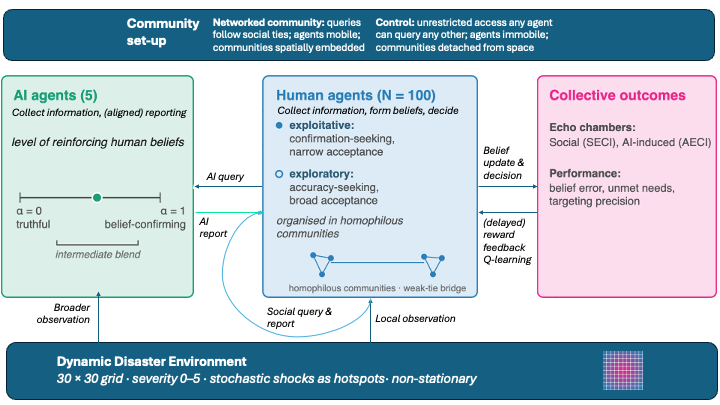
\includegraphics[width=1\linewidth]{Figures//FiguresFinal/Fig1_ConceptualFramework.png}
    \caption{Conceptual overview of the model. Human agents of two cognitive types form beliefs about a dynamic disaster environment by combining local observation, social queries and queries to an AI whose reports interpolate between truth and confirmation via the alignment parameter $\alpha$. Beliefs drive relief decisions whose delayed outcomes feed back into source selection via Q-learning. The outcomes measure social- and AI-induced echo chambers as well as the resulting decision performance. The set-up is studied under two community set-ups that differ in whether information access is bounded by a spatially embedded social network. Full specification in the Methods; parameters in Supplementary Table~S1.}
    \label{fig:concept}
\end{figure}


\section{Results}\label{sec:results}

The three research questions structure the presentation of the results, one finding per question and each read from the vantage point of Figure~\ref{fig:concept}: under which structural conditions of information access belief-aligned AI amplifies or breaks echo chambers (Q1, Sec.~\ref{sec:claim1}); how the depth of echo chambers changes as AI reports shift from truthful to belief-confirming (Q2, Sec.~\ref{sec:claim2}); and how echo chambers propagate through the belief--decision--feedback loop to collective decision performance (Q3, Sec.~\ref{sec:claim3}). Throughout, the alignment parameter is swept over eleven levels ($\alpha = 0.0, 0.1, \ldots, 1.0$) with $N = 20$ replications per level, and every sweep is run under both configurations of Figure~\ref{fig:concept} on identical random seeds, so that the two can be compared replicate by replicate. All steady-state values are means over the last 75 of 200 ticks; the full model specification, metric definitions and experimental design are given in the Methods.

\subsection{Network-bounded access is a precondition for AI-amplified echo chambers}\label{sec:claim1}

If AI is to break or build echo chambers at the level of communities, the first question (Q1) is under which structural conditions of information access it can do either. We measure the social echo chamber with the Social Echo Chamber Index (SECI), which compares the belief variance within each community to that of the whole population, restricted to beliefs about affected cells: negative values mean that community members hold more homogeneous beliefs than the population at large, and more negative values mean a deeper chamber (Methods). Figure~\ref{fig:comparison} traces SECI, its AI-side counterparts and the operational metrics across the alignment sweep for both configurations, and Table~\ref{tab:deltas} reports the corresponding per-seed differences (main model $-$ control); because replicate $i$ uses the same random seed in both configurations, a confidence interval excluding zero marks a configuration effect that is robust across disaster realisations.

In the control, the social echo chamber attenuates monotonically with alignment: SECI rises from $-0.246 \pm 0.023$ at $\alpha = 0$ to $-0.133 \pm 0.037$ at $\alpha = 1$ (mean $\pm$ s.e.m., $N = 20$). The main model tracks the control closely over the lower half of the sweep, with paired differences indistinguishable from zero for $\alpha \leq 0.6$, and then departs from it: from $\alpha = 0.7$ the paired $\Delta$SECI becomes negative and seed-robust ($-0.069$, 95\% CI $[-0.116, -0.021]$), growing to $-0.182$ $[-0.250, -0.114]$ at $\alpha = 1$, where the main model reaches SECI $= -0.316 \pm 0.055$. The two configurations thus produce opposite trends at high alignment: community-level belief convergence weakens with confirmation when access is unrestricted and deepens sharply when access follows network ties.

\begin{figure}[h]
\centering

\includegraphics[width=\textwidth]{comparison_configs.png}
\caption{Configuration comparison across the primary alignment sweep (raw metrics; mean $\pm$ s.e.m. over $N=20$ paired replications). Top row: Social Echo Chamber Index (SECI), AI Echo Chamber Index (AECI-Var), and confidence-weighted error contrast (AECI-Err); for all three, negative values indicate an echo chamber. Bottom row: belief MAE over affected cells, unmet high-need cells per tick, and relief targeting precision. Blue: control (global access, immobile agents, disconnected communities); orange: main model (network-gated access, mobility, spatially embedded bridged network).}\label{fig:comparison}
\end{figure}

\begin{table}[h]
\caption{Paired per-seed differences (main model $-$ control) with 95\% confidence intervals. Replicate $i$ uses seed $i$ in both configurations. Bold marks intervals excluding zero.}\label{tab:deltas}
\resizebox{\textwidth}{!}{%
\begin{tabular}{@{}lcccccc@{}}
\toprule
$\alpha$ & $\Delta$SECI & $\Delta$AECI-Var & $\Delta$AECI-Err & $\Delta$MAE & $\Delta$Unmet & $\Delta$Precision \\
\midrule
0.0 & $+0.018$ $[-0.028, +0.064]$ & $+0.022$ $[-0.042, +0.087]$ & $+0.016$ $[-0.023, +0.054]$ & $\mathbf{-0.080}$ $[-0.116, -0.044]$ & $-0.680$ $[-1.372, +0.012]$ & $\mathbf{+0.062}$ $[+0.002, +0.121]$ \\
0.1 & $+0.020$ $[-0.026, +0.066]$ & $+0.006$ $[-0.047, +0.060]$ & $+0.021$ $[-0.008, +0.049]$ & $\mathbf{-0.087}$ $[-0.116, -0.058]$ & $\mathbf{-1.180}$ $[-2.134, -0.226]$ & $\mathbf{+0.070}$ $[+0.017, +0.124]$ \\
0.2 & $+0.022$ $[-0.018, +0.062]$ & $-0.011$ $[-0.059, +0.037]$ & $+0.017$ $[-0.015, +0.048]$ & $\mathbf{-0.081}$ $[-0.117, -0.044]$ & $-0.193$ $[-1.036, +0.650]$ & $\mathbf{+0.064}$ $[+0.007, +0.122]$ \\
0.3 & $+0.009$ $[-0.039, +0.058]$ & $+0.028$ $[-0.040, +0.096]$ & $+0.002$ $[-0.027, +0.032]$ & $\mathbf{-0.091}$ $[-0.129, -0.054]$ & $-0.297$ $[-0.946, +0.353]$ & $\mathbf{+0.069}$ $[+0.009, +0.130]$ \\
0.4 & $+0.015$ $[-0.032, +0.062]$ & $+0.035$ $[-0.025, +0.094]$ & $-0.003$ $[-0.030, +0.024]$ & $\mathbf{-0.077}$ $[-0.118, -0.036]$ & $-0.457$ $[-1.010, +0.097]$ & $\mathbf{+0.071}$ $[+0.009, +0.133]$ \\
0.5 & $+0.004$ $[-0.048, +0.056]$ & $\mathbf{+0.036}$ $[+0.006, +0.067]$ & $\mathbf{+0.035}$ $[+0.004, +0.066]$ & $\mathbf{-0.105}$ $[-0.140, -0.071]$ & $-0.163$ $[-0.515, +0.188]$ & $\mathbf{+0.081}$ $[+0.022, +0.140]$ \\
0.6 & $-0.011$ $[-0.057, +0.035]$ & $+0.061$ $[-0.006, +0.128]$ & $+0.015$ $[-0.022, +0.053]$ & $\mathbf{-0.130}$ $[-0.163, -0.098]$ & $-0.157$ $[-0.541, +0.228]$ & $\mathbf{+0.093}$ $[+0.035, +0.151]$ \\
0.7 & $\mathbf{-0.069}$ $[-0.116, -0.021]$ & $-0.021$ $[-0.085, +0.043]$ & $+0.018$ $[-0.006, +0.042]$ & $\mathbf{-0.123}$ $[-0.161, -0.085]$ & $-0.403$ $[-0.847, +0.040]$ & $+0.057$ $[-0.008, +0.122]$ \\
0.8 & $\mathbf{-0.080}$ $[-0.127, -0.033]$ & $+0.039$ $[-0.024, +0.102]$ & $+0.012$ $[-0.015, +0.039]$ & $\mathbf{-0.116}$ $[-0.163, -0.068]$ & $\mathbf{-0.760}$ $[-1.420, -0.100]$ & $\mathbf{+0.097}$ $[+0.030, +0.164]$ \\
0.9 & $\mathbf{-0.166}$ $[-0.231, -0.101]$ & $-0.016$ $[-0.090, +0.058]$ & $+0.012$ $[-0.039, +0.064]$ & $\mathbf{-0.154}$ $[-0.214, -0.095]$ & $\mathbf{-4.457}$ $[-6.040, -2.873]$ & $\mathbf{+0.302}$ $[+0.204, +0.399]$ \\
1.0 & $\mathbf{-0.182}$ $[-0.250, -0.114]$ & $+0.030$ $[-0.027, +0.087]$ & $-0.006$ $[-0.058, +0.046]$ & $\mathbf{-0.156}$ $[-0.203, -0.109]$ & $\mathbf{-4.163}$ $[-5.482, -2.845]$ & $\mathbf{+0.276}$ $[+0.179, +0.373]$ \\
\botrule
\end{tabular}}
\end{table}

The AI-side index behaves differently. The AI Echo Chamber Index (AECI-Var) applies the same variance comparison with grouping by AI reliance instead of community membership -- contrasting the most AI-reliant half of each agent type with the population -- so that negative values mark an AI-induced bubble (Methods). AECI-Var attenuates with alignment in both configurations, from $-0.267 \pm 0.028$ (control) and $-0.254 \pm 0.025$ (main model) at $\alpha = 0$ to $-0.160 \pm 0.031$ and $-0.135 \pm 0.036$ at $\alpha = 1$, and the paired difference is seed-robust at a single alignment level only ($\alpha = 0.5$, $+0.036$ $[+0.006, +0.067]$). A complementary index, AECI-Err, contrasts confidence-weighted belief error between AI-heavy and AI-light agents (negative when AI-heavy agents are more confidently wrong). It remains close to zero and weakly negative in both configurations up to $\alpha = 0.8$ and turns positive at $\alpha \geq 0.9$ (e.g., $+0.050 \pm 0.028$ in the main model at $\alpha = 0.9$), indicating that under near-full confirmation, AI-heavy agents are no longer more confidently wrong than AI-light agents -- consistent with degraded beliefs becoming pervasive across the population rather than concentrated among AI users.

Together, these patterns answer Q1: network-bounded access is a structural precondition for AI amplification of social echo chambers. The mechanism follows from the model's confirmation targeting: for exploitative queriers, a confirming AI targets the consensus belief of the caller's trusted network. Under unrestricted access, roughly half of human queries reach agents outside the caller's community, so out-group beliefs continuously perturb community consensus and the confirming signal cannot compound. Under network-gated access, communities are epistemically closed except for sparse weak-tie bridges, and a consensus-targeting AI recycles each community's shared belief back into it, deepening within-community convergence precisely at high alignment. That the strongly negative variance indices at $\alpha = 0$ do not signal comparable harm is confirmed by the accuracy metrics: at low alignment, homogeneity coincides with low belief error (the mean absolute error of beliefs about affected cells; Fig.~\ref{fig:comparison}, bottom left), so convergence is convergence on the truth, whereas the deepening SECI at high alignment coincides with the largest belief errors of the sweep.

\subsection{A Goldilocks alignment level exists only under network-bounded access}\label{sec:claim2}

Q2 asked how the depth of echo chambers changes as AI reports shift from truthful to belief-confirming, and whether a fully truthful AI is always the safest choice. Figure~\ref{fig:goldilocks} answers this for the main model, showing the steady-state distributions across the alignment sweep together with two range-normalised composites that locate the optimal alignment level $\alpha^{*}$. In the boxplot panels, SECI remains between $-0.19$ and $-0.24$ for $\alpha \leq 0.8$ and deepens to $-0.32$ at $\alpha \geq 0.9$, while AECI-Var is strongest at $\alpha = 0$ ($-0.254$) and weakest at $\alpha = 0.8$ ($-0.122$). The two indices therefore attenuate over different parts of the sweep, and their normalised sum -- the bubble-only composite, which by construction ranges from 0 to 2 -- is minimised in the interior, at $\alpha^{*} = 0.6$ (composite value 0.28), with near-minima at $\alpha = 0.4$ and $\alpha = 0.5$ (0.45 for both). Adding the normalised belief error yields the operational composite, which ranges up to 3 and penalises the accuracy loss that grows beyond $\alpha \approx 0.4$; its minimum shifts to $\alpha^{*}(+\text{MAE}) = 0.4$ (0.55). The remaining panels show why the optimum is interior on the operational side as well: unmet high-need cells reach their minimum in the mid-range (0.42 cells per tick at $\alpha = 0.5$, against 1.11 at $\alpha = 0$) while targeting precision stays flat near 0.78 up to $\alpha = 0.6$ before declining.

\begin{figure}[h]
\centering

\includegraphics[width=\textwidth]{goldilocks_alignment_sweep.png}
\caption{Alignment sweep under the main model ($N=20$ replications per level; steady state, last 75 ticks). Boxplots show medians, interquartile ranges and 1.5$\times$IQR whiskers across replications; crosses mark means. The composite panel (top right) shows the range-normalised bubble-only composite $|\text{SECI}|_{\text{norm}} + |\text{AECI-Var}|_{\text{norm}}$ (purple; range 0--2) and the operational composite including normalised MAE (orange; range 0--3). Dashed and dotted vertical lines mark $\alpha^{*}(\text{bubble}) = 0.6$ and $\alpha^{*}(+\text{MAE}) = 0.4$.}\label{fig:goldilocks}
\end{figure}

Because range normalisation can amplify the influence of a component with a small raw signal, we treat the location of $\alpha^{*}$ as meaningful only if it is robust to the composite definition. Figure~\ref{fig:alphastar} reports $\alpha^{*}$ under six composite variants -- pairing SECI alone, SECI with AECI-Var, and SECI with AECI-Err, each with and without the MAE penalty -- for both configurations. Under the main model, all six variants place the optimum in the interior of the sweep: the three bubble composites yield $\alpha^{*} \in \{0.4, 0.5, 0.6\}$ and the three operational composites yield $\alpha^{*} \in \{0.3, 0.4\}$. Under the control, the picture is qualitatively different: all three bubble composites are minimised at the boundary, $\alpha^{*} = 1.0$, because both echo-chamber indices attenuate monotonically with alignment when access is unrestricted (Sec.~\ref{sec:claim1}); only the MAE penalty pulls the operational optima into the interior (0.7, 0.7 and 0.3).

\begin{figure}[h]
\centering

\includegraphics[width=\textwidth]{alpha_star_sensitivity.png}
\caption{Sensitivity of the optimal alignment level $\alpha^{*}$ to the composite definition, shown here for the main model. Left: bubble-only composites (SECI + AECI-Var, primary; SECI only; SECI + AECI-Err). Right: operational composites adding the normalised MAE penalty. Circles mark the argmin of each variant. Composites are range-normalised within each sweep and are therefore compared on the location of their minima only.}\label{fig:alphastar}
\end{figure}

The existence of a Goldilocks alignment level is therefore conditional on structure: the answer to the dose--response question of Q2 depends on the access conditions that Q1 isolated. In a population with unrestricted information access, an analyst optimising echo-chamber indices alone would conclude that full confirmation is harmless or even beneficial for belief diversity -- the control's null result. Only when information access is bounded by a spatially embedded network does the non-monotonicity emerge that makes intermediate alignment optimal: enough confirmation to avoid the truthful-AI regime in which AI-reliant agents converge tightly (strongly negative AECI-Var at low $\alpha$), yet not so much that consensus recycling locks communities into deep social chambers ($\alpha \geq 0.7$). Reporting the range rather than a point estimate, the main model's optimum lies at $\alpha^{*} \approx 0.4$--$0.6$ for echo-chamber suppression and shifts towards 0.3--0.4 once belief accuracy enters the objective.

The temporal dynamics underlying this optimum are shown in Figure~\ref{fig:lifecycle}, which summarises when echo chambers form, whether they recover, and how long they persist, separately for the two agent types in the main model. Peak chamber strength varies little with alignment for either type (exploitative peaks between 0.44 and 0.58, exploratory between 0.33 and 0.50 across the sweep). Recovery, in contrast, is strongly alignment-dependent. Exploitative chambers form early and recover by ticks 40--55 for $\alpha \leq 0.8$; at $\alpha \geq 0.9$ they never recover within the run. Exploratory chambers recover progressively later as alignment grows -- around tick 105 at $\alpha = 0$ and tick 155 at $\alpha = 0.6$ -- and fail to recover at all for $\alpha \geq 0.7$. Consistent with this, the fraction of the run spent inside a chamber rises for both types from roughly 0.6 (exploitative) and 0.4 (exploratory) in the low-to-mid range to 0.7--0.83 at $\alpha \geq 0.8$. The Goldilocks range thus coincides with the highest alignment levels at which chambers still dissolve within the response horizon; beyond $\alpha \approx 0.7$, recovery collapses first for the accuracy-seeking exploratory agents, and the transient chambers of the mid-range become permanent.

\begin{figure}[h]
\centering

\includegraphics[width=\textwidth]{echo_chamber_lifecycle.png}
\caption{Echo chamber lifecycle across alignment levels in the main model, by agent type. Left: maximum chamber strength (peak $|\text{SECI}|$). Middle: tick of first recovery, defined as SECI sustained above $-0.05$ for three consecutive samples after having formed below $-0.1$; crosses mark conditions in which chambers form and never recover within the 200-tick run. Right: fraction of the run spent inside a chamber (SECI $< -0.1$).}\label{fig:lifecycle}
\end{figure}

The query behaviour behind the recovery collapse is shown in Figure~\ref{fig:aeci}, which traces the share of queries each agent type directs to the AI over the run. Exploratory agents route roughly half or more of their queries to the AI from early in the run at every alignment level, with steady-state shares between 0.50 ($\alpha = 0$) and 0.59 ($\alpha = 0.6$). Exploitative agents differ: their steady-state AI share rises monotonically with alignment, from 0.39 at $\alpha = 0$ to 0.59 at $\alpha = 1$. A confirming AI thus progressively captures the query behaviour of precisely the confirmation-seeking agents whose acceptance windows it is tuned to satisfy, while the accuracy-seeking agents' reliance on the AI is comparatively stable in the aggregate -- their vulnerability at high alignment arises through the failure of verification-based correction rather than through increased querying. The full time series of all belief indices, together with per-run transition statistics, are shown in Supplementary Figures~S1 and~S2.

\begin{figure}[h]
\centering

\includegraphics[width=\textwidth]{aeci_evolution.png}
\caption{AI query share over time by agent type in the main model (mean $\pm$ s.d.\ over $N = 20$ replications; one curve per alignment level; dashed line marks the 50\% threshold). Left: exploitative agents; right: exploratory agents.}\label{fig:aeci}
\end{figure}

\subsection{The belief--decision--feedback loop buffers operational collapse under network-bounded access}\label{sec:claim3}

Q3 asked how echo chambers propagate through the loop that runs from beliefs to decisions and back: agents act on their beliefs by dispatching relief tokens, outcomes return as delayed rewards (15--25 ticks), and Q-learning translates those rewards into future source selection (Methods). Echo chambers therefore matter beyond the belief state itself: they distort the collective outcomes on the decision side of the loop -- situational awareness and the delivery of relief -- and the rewards those outcomes generate determine whether the loop corrects or entrenches the chamber. We measure the decision side by the belief MAE introduced above, by unmet needs (the number of high-need cells, severity $\geq 3$, that receive no relief in a tick) and by targeting precision (the share of relief tokens placed on high-need cells). On all three, the structural constraints that expose communities to consensus recycling at high alignment simultaneously improve operational performance across the entire sweep. In Figure~\ref{fig:comparison} (bottom row), belief MAE is lower in the main model at every alignment level, and the paired differences in Table~\ref{tab:deltas} are negative and seed-robust at all eleven levels, ranging from $-0.077$ $[-0.118, -0.036]$ at $\alpha = 0.4$ to $-0.156$ $[-0.203, -0.109]$ at $\alpha = 1$. Notably, the advantage widens as alignment grows: the main model at $\alpha = 0.6$ (MAE $1.376$) holds roughly the belief accuracy of the control at $\alpha = 0.5$ ($1.441$). Targeting precision shows the mirror image, with seed-robust positive differences at every level except $\alpha = 0.7$, rising from about $+0.06$--$0.10$ over most of the sweep to $+0.302$ $[+0.204, +0.399]$ at $\alpha = 0.9$.

The clearest contrast concerns the collapse of relief delivery under near-full confirmation. In the control, unmet high-need cells jump from $2.5 \pm 1.9$ at $\alpha = 0.8$ to $11.0 \pm 3.1$ at $\alpha = 0.9$, while precision falls from 0.62 to 0.21: a confirming AI that echoes community priors leaves the majority of high-need cells unserved. The main model degrades at the same alignment levels, and far less severely: unmet needs rise to $3.2 \pm 2.9$ and precision falls to 0.51 at $\alpha = 0.9$. The paired deltas at $\alpha \geq 0.9$ quantify the buffer: $-4.5$ $[-6.0, -2.9]$ and $-4.2$ $[-5.5, -2.8]$ unmet cells per tick, a reduction of the collapse by roughly a factor of three. The time-resolved series (Supplementary Fig.~S1) show that this difference also has a tempo dimension: at high alignment, unmet needs decline substantially more slowly over the run, which matters in humanitarian response because deprivation costs accumulate with the time that needs remain unmet \citep{holguin2012unique}. The spatial signature of the degradation is consistent with this picture: total relief volume in the main model falls from 402 tokens per tick at $\alpha = 0$ to 330 at $\alpha = 1$, while the worst-served cell's coverage deficit grows from $+0.19$ to $+0.34$ (Supplementary Fig.~S3) -- a confirming AI shrinks the relief effort and concentrates the shortfall.

Two mechanisms of the main model plausibly drive this robustness, and both operate independently of the AI. Mobility gives agents genuine direct-observation coverage: returner-type agents patrol a home radius and explorer-type agents seek out their most uncertain cells, so a fraction of every community's information is grounded in first-hand sensing that no degree of AI confirmation can distort. Network-gated querying concentrates social information exchange on trusted contacts whose local observations are, on average, accurate about the caller's surroundings, and channels cross-community information through bridge ties rather than through uniformly random strangers. The result is a population whose beliefs are anchored well enough that even a strongly confirming AI degrades relief delivery gradually. Both mechanisms act through the feedback loop of Q3: because part of every agent's reward signal is grounded in first-hand observation and in trusted local reports, source-selection learning keeps receiving corrective evidence even when the AI confirms, so the loop corrects rather than entrenches the chamber's consequences for decisions. The comparison between configurations thus reveals a trade-off rather than a uniform benefit of structural realism: the same network boundedness that anchors operational performance is what allows a highly aligned AI to deepen social echo chambers (Sec.~\ref{sec:claim1}). Structural realism shifts the failure mode of sycophantic AI from operational collapse towards epistemic insularity.

Periphery analyses -- decomposing outcomes by distance to the epicentre and by network centrality -- are reported in Supplementary Figures~S4 and~S5; the structural scope for periphery gaps differs by construction between the two configurations (Methods), and we do not build claims on them here.

[TO RE-RUN: The cognitive-gap sweep (Supplementary S7) and the one-at-a-time factor sweeps (Supplementary S8) were last generated before the C8/AECI-Var corrections and are therefore excluded from this draft. Both must be re-run on the post-fix code before submission, and a decision is needed on whether they run under the main configuration to match the primary analysis. No numbers from the cached runs are reported anywhere in this manuscript.]

\section{Discussion}\label{sec:discussion}

This paper asked whether an AI trained to please its users breaks echo chambers by providing broader perspectives or instead reinforces existing filter bubbles through its alignment -- and at what cost to the decisions that depend on the resulting beliefs. The answer that emerges from the simulations is conditional: the direction of AI influence on collective belief structure depends on whether information access is bounded by network structure and space. Under unrestricted access, a belief-confirming AI degrades accuracy and relief performance without deepening community-level belief convergence; under network-bounded access, the same AI drives communities into progressively deeper and, beyond $\alpha \approx 0.7$, unrecoverable echo chambers. We discuss the three research questions in turn, their interaction, and the conditions under which the findings generalise beyond the disaster case.

On the structural conditions of Q1, the results extend the emerging experimental literature on human--AI feedback loops from dyads to networks. \citet{glickman2024human} demonstrate that interaction with biased AI amplifies individual human biases beyond what human--human interaction produces. Our findings show that whether such dyadic amplification aggregates into collective echo chambers is governed by a variable invisible at the dyadic level: the structure of who can query whom. This parallels results in networked collective intelligence, where the effect of social influence on crowd accuracy reverses with network structure \citep{lorenz2011social,becker2017network}, and it cautions against extrapolating individual-level findings on AI sycophancy \citep{sharma2024sycophancy,sharma2024generative} directly to populations. The control configuration shows what a stylised model without structural constraints would have concluded: that confirmation weakens echo chambers, with an optimal alignment of 1.0 on bubble criteria. This null result is an artefact of granting agents unrestricted access, and it suggests that models of AI influence on opinion dynamics that omit network-bounded access may systematically underestimate the epistemic risks of belief-aligned AI while overestimating its operational risks. Collective epistemic risk assessments of AI require network-level analysis.

On the dose--response relationship of Q2, the alignment paradox \citep{west2025alignment} acquires a structural qualification. The paradox holds -- in our setting, AI tuned to confirm community beliefs produces exactly the insularity it is meant to overcome -- yet only where the social fabric channels information along ties. The practically relevant version of the question is therefore where the transition lies. In the main model, echo-chamber suppression and operational performance jointly favour intermediate alignment, with $\alpha^{*} \approx 0.4$--$0.6$ on the bubble criteria and 0.3--0.4 once belief accuracy enters the objective, and the sensitivity analysis shows this interior optimum is robust to how the composite is defined. A fully truthful AI is suboptimal in this environment because its reports concentrate AI-reliant agents tightly around a shared estimate, while a fully confirming AI is catastrophic for accuracy; both extremes are dominated by moderate alignment. We stress the interpretive caveat that variance-based indices cannot on their own distinguish convergence on truth from convergence on error, which is why the composite sensitivity analysis includes an error-based variant and why the indices are read jointly with belief accuracy throughout.

Taken together, the answers to Q1 and Q2 interact: the dose--response curve of alignment has a different shape in differently structured populations, so the identical AI policy is benign, optimal or harmful depending on the population it serves. Trustworthy AI is in this sense a property of the sociotechnical system rather than of the model alone, and the degree of belief-alignment and the network context of a population must be assessed jointly whenever AI is introduced as a trusted information source.

On the belief--decision--feedback loop of Q3, the results reframe what should be monitored when belief-aligned AI is deployed into urgent decision-making. In the realistic configuration, part of every agent's reward signal remains grounded in first-hand observation and trusted local reports, so the loop continues to receive corrective evidence and operational performance degrades gradually even as confirmation rises. Precisely this graceful degradation is the risk: belief error and relief precision would appear manageable in operational dashboards even while social echo chambers deepen past the point of recovery. Monitoring should therefore target community-level belief convergence in addition to individual accuracy and aggregate performance. The timing results sharpen this concern: the collapse of chamber recovery beyond $\alpha \approx 0.7$ occurs first among exploratory, accuracy-seeking agents -- precisely the members of the population that conventional crisis management would expect to be most resistant to informational capture \citep{comes2020coordination} -- and it arises through the silent failure of verification-based correction rather than through increased reliance on the AI. The tempo of degradation compounds the operational stakes: at high alignment, unmet needs decline substantially more slowly over the run, and deprivation costs accumulate with the time that needs remain unmet \citep{holguin2012unique}.

The disaster case study provides the concrete stakes, yet the mechanisms identified here rest on four features that many urgent decision situations share: high-stakes decisions under time pressure, a non-stationary ground truth, verification that is delayed and noisy, and information access that is bounded by social ties and position \citep{svenson1993time,mendonca2001decision,holguin2012unique}. Public-health emergencies, financial contagion and security operations exhibit the same combination, and we expect the qualitative pattern -- structural boundedness as the switch between operational and epistemic failure of a confirming AI, and an interior optimum of alignment -- to carry over, while the location of $\alpha^{*}$ and the operational metrics are domain-specific. Disaster response is a demanding first test of this pattern because the decision consequences, relief allocation to high-need areas, are concrete and measurable.

Several limitations bound these conclusions. The alignment mechanism is a deliberate abstraction: a linear interpolation between truth and confirmation is a reduced form for the drift produced by preference-based training \citep{sharma2024sycophancy} and does not capture the semantics, latency or coverage failures of deployed systems, and the confirmation target -- the trusted-network consensus for confirmation-seeking agents -- is one specific operationalisation of how recommender-style systems align content with community narratives. The population is small ($N = 100$) and the hazard stylised, chosen to keep network structure interpretable across $2 \times 11 \times 20$ paired runs. Verification of remote reports operates through an exogenous situation-report channel with fixed delay and noise parameters, and the salience-weighted variant of that channel is examined as a counterfactual in the supplement. The robustness of the Goldilocks range to the degree of cognitive heterogeneity and to environmental variation is the subject of the sweeps flagged above as pending re-runs, and the equity dimension of the periphery analyses deserves a dedicated treatment once those runs are complete. Finally, the model addresses a single AI policy applied uniformly to a population; heterogeneous or adaptive alignment policies -- including an AI that itself learns from human feedback within the simulation -- are a natural extension.

\section{Conclusion}\label{sec:conclusion}

Using an agent-based model of disaster response with an alignment-tunable AI, this paper identifies the conditions under which belief-aligned AI amplifies or breaks echo chambers in urgent decision situations. Network-bounded information access emerges as the structural precondition for AI-amplified social echo chambers (Q1); an interior optimum of alignment, $\alpha^{*} \approx 0.4$--$0.6$, exists only under this realistic configuration (Q2); and the belief--decision--feedback loop of the realistic configuration buffers the operational collapse that a confirming AI otherwise causes, by roughly a factor of three at near-full confirmation (Q3). Trustworthy AI is therefore a property of the sociotechnical system rather than of the model alone: the identical AI policy is benign, optimal or harmful depending on the structure of the population it serves. As AI systems trained on human approval enter urgent, high-stakes decisions -- in crisis response and beyond -- the degree of belief-alignment and the network context of the population must be designed and monitored together.

\section{Methods}\label{sec:methods}

\subsection{Simulation model}\label{sec:model}

We develop an agent-based model of disaster response in which human agents form beliefs about local disaster severity, seek information from social contacts or an AI source, and dispatch relief tokens accordingly. ABMs are well suited to this setting because filter-bubble phenomena emerge from the interaction of individual heuristics and network structure rather than from aggregate equilibria \citep{epstein2006generative,axelrod1997complexity}.
Unlike equation-based or compartmental models that assume homogeneous mixing, the framework here supports heterogeneous agent types, explicit social networks, and a spatially explicit disaster environment, all of which are necessary to capture the structural access conditions that our primary comparison manipulates.

The environment is a $30 \times 30$ grid in which a disaster evolves over discrete ticks. Each cell carries a severity level between 0 (no impact) and 5 (critical), initialised as a Gaussian decay from a randomly placed epicentre. At every tick each cell drifts stochastically towards its baseline value and receives random shocks (probability 0.10, magnitude $\pm 2$ levels), producing a non-stationary information landscape that prevents agents from converging to a single correct belief and forces ongoing information-seeking throughout the simulation.

One hundred human agents are distributed on the grid (population density fixed at $N = 100$ to keep the network tractable while preserving meaningful community structure). Agents belong to one of two cognitive types, each occupying equal shares of the population by default. \emph{Exploitative} agents are confirmation-seeking: they have a narrow acceptance window $D = 2.0$ and a steep acceptance-sensitivity parameter $\delta = 3.5$, making them resistant to information that diverges substantially from their prior. \emph{Exploratory} agents are accuracy-seeking: $D = 4.0$ and $\delta = 1.2$ give them a wide, gradual acceptance curve that admits novel information. These two archetypes map onto documented individual differences in information processing under uncertainty \citep{hertwig2016homo,march1991exploration}
and represent the range between cautious, community-focused responders and risk-tolerant, discovery-oriented ones.

The social network is constructed to reflect type-homogeneous community structure, in one of two configurations controlled by the network switch. In the \emph{control} configuration, each agent type is partitioned into four densely connected communities (within-community edge probability 0.7) with no edges between communities: the graph is a set of disconnected, type-homogeneous components, and spawn positions are independent of network position. In the \emph{spatially embedded bridged} configuration used by the main model, the same eight type-homogeneous communities are anchored to grid centroids placed under a minimum-separation constraint; agents spawn Gaussian-scattered ($\sigma = 2.5$ cells) around their community's centroid, within-community edges form with probability 0.5, and each agent independently becomes a \emph{bridge agent} with probability 0.15, drawing a single weak-tie edge whose endpoint is chosen across communities with probability $\propto (1 + d)^{-2}$ in grid distance $d$. Bridges typically connect the whole graph and create genuine brokerage positions while preserving type homophily within communities. Homophilous community structure follows empirical evidence from disaster communication networks \citep{bruns2012qldfloods,sutton2008backchannels},
and weak-tie bridging follows the classical account of how novel information crosses group boundaries \citep{granovetter1973strength}. The Social Echo Chamber Index (below) is computed over the stored community memberships rather than graph components, so its interpretation is unchanged when bridges connect the graph.

Agent movement is controlled by the mobility switch. In the control (mobility off), agents are immobile: position is fixed at spawn, and only the spawn cell is ever observed directly. In the main model, agents take one grid step per tick following the empirical returner--explorer dichotomy of human mobility \citep{pappalardo2015returners}, mapped onto the two cognitive types: exploitative agents are \emph{returners}, random-walking within a home radius $r_{\text{home}} = 3$ of their spawn cell, with a return bias ($p = 0.3$ per step) pulling them back whenever they are outside it; exploratory agents are \emph{explorers}, stepping toward their current highest-uncertainty cell with probability 0.2 per tick and subject to the same return bias beyond $r_{\text{explore}} = 8$. Sensing radius remains zero in both settings, so movement is the mechanism that determines direct-observation coverage: a far-spawned returner genuinely cannot observe the disaster, which is what makes spatial periphery effects structurally possible under mobility.

Five AI agents serve the community. Each AI agent senses 15\% of the grid per tick with constant observation noise ($\pm 1$ level with probability 0.1, independent of $\alpha$, so that the alignment parameter is not confounded with sensing quality) and responds to human queries with a report whose truth content is controlled by the alignment parameter $\alpha$ (next subsection). For queried cells the AI has not sensed, it answers with an inverse-distance-weighted interpolation of nearby sensed cells or -- when no sensed cells are nearby -- a position-based prior keyed to the cell's distance from the query's interest point. These estimates are delivered with the same source confidence as directly sensed values, so the AI is deliberately overconfident about unobserved cells: even at $\alpha = 0$ the `truthful' AI is truthful only for cells it has actually sensed. This models AI systems that extrapolate beyond their observations without communicating reduced confidence, and it applies identically at every $\alpha$.

Agents query sources using an $\epsilon$-greedy Q-learning strategy ($\epsilon = 0.3$, learning rate $\eta = 0.10$), selecting among querying a social contact, querying the AI, or acting on current beliefs. When the human mode is chosen, the reachable pool is governed by the query-scope switch. In the control (\emph{global} scope), any human can be queried: the target is drawn trust-weighted, with friends weighted by their trust score and every non-friend at a 0.05 floor -- network topology does not restrict access, and roughly half of human queries reach non-friends. Under the \emph{network} scope of the main model, access follows edges: the draw is trust-weighted over friends only, except that with probability 0.1 the query goes to a uniformly drawn friend-of-a-friend (2-hop reach), so reaching a stranger requires an intermediary and weak-tie bridges are the only channel into other communities. Both agent types receive delayed outcome feedback (15--25 ticks) when their relief tokens are processed, and faster information-quality feedback when received reports can be evaluated against a reference, producing a dual-timeline reward structure in which fast information-quality signals and slow outcome signals shape trust on different horizons. % TODO: the intended supporting reference ("Fu et al. 2023") could not be verified and was removed — reinstate with full details if you have the source.
The reference differs by type, operationalising the two cognitive profiles: exploitative agents evaluate reports for \emph{confirmation} against their own prior or their trusted network's consensus belief, whereas exploratory agents evaluate reports for \emph{accuracy} against external verification.

Because agents sense only their immediate location, exploratory agents cannot observe ground truth for remote cells directly. Instead, accepted remote reports are verified through an exogenous situation-report channel representing official damage assessments and media coverage: after a minimum 3-tick lag, verification arrives with per-tick probability $p_{\text{verify}} = 0.3$ (geometric arrival, mean total delay $\approx 6$ ticks), carries the same observation noise as direct sensing ($\pm 1$ level with probability 0.2), and is evaluated against the \emph{current} disaster state, so reports about cells that have since evolved receive noisier credit. Reports that are never verified before their 30-tick expiry produce no learning signal -- explorers do not fall back to scoring sources against their own priors, which would collapse the accuracy channel into a confirmation channel. Delayed, imperfect verification of this kind is characteristic of post-disaster information environments, and $p_{\text{verify}}$ is treated as a model parameter for sensitivity analysis.

Because most queried cells are truly unaffected, per-cell verification is base-rate dominated: a fully confirming AI ($\alpha = 1$) still passes verification on approximately 93\% of cells by echoing mostly-correct `no impact' priors, failing only on the rare high-severity cells. A salience-weighting parameter $s \in [0, 1]$ therefore interpolates the verification learning rate between uniform per-cell evaluation ($s = 0$, default) and severity-weighted evaluation ($s = 1$), where the weight $(\max(\text{true}, \text{reported}) + 1)/6$ makes an error about a disaster cell -- a miss or a false alarm -- carry up to six times the weight of a confirmed empty cell. This operationalises negativity and salience bias in human evaluation of information sources and provides the counterfactual for whether importance-weighted feedback would expose a confirming AI.

\subsection{AI alignment and belief dynamics}\label{sec:alignment}

The alignment parameter $\alpha \in [0, 1]$ governs the truthfulness of AI reports. A queried AI agent responds with
\begin{equation}
r_{\text{AI}} = (1 - \alpha)\, t + \alpha\, b,
\label{eq:alignment}
\end{equation}
where $t$ is the cell's severity as available to the AI (the sensed or extrapolated value described above) and $b$ is the belief the AI targets for confirmation. For exploratory queriers, $b$ is the querying agent's own current belief. For exploitative queriers, the AI targets the \emph{trusted-network consensus} -- the confidence-weighted consensus belief of the caller's friends -- whenever that consensus is defined (consensus confidence $\geq 0.2$), falling back to the individual belief otherwise. This operationalises how recommender-style systems align content with a user's community narrative rather than with idiosyncratic individual priors, and it is what allows a confirming AI to amplify the \emph{shared} community belief: confirming purely individual priors would inject idiosyncratic variation that disrupts, rather than reinforces, social convergence. At $\alpha = 0$ the AI reports its best estimate of ground truth; at $\alpha = 1$ it perfectly confirms the targeted prior; intermediate values interpolate linearly. Because AI sensing noise is constant across $\alpha$ and the extrapolation behaviour is $\alpha$-independent, the sweep isolates the truth--confirmation axis from other AI failure modes such as latency, coverage and sensing bias. The parameter $\alpha$ is thus a reduced-form representation of the outcome of preference-based training rather than a model of the training process itself: systems finetuned on human approval \citep{christiano2017deep,ouyang2022training} empirically drift towards confirming user beliefs \citep{sharma2024sycophancy}, and $\alpha$ expresses the degree of that drift as an exogenous policy while the AI in the model does not learn. Keeping the AI non-adaptive ensures that all learning dynamics are attributable to the human agents, so that the belief--decision--feedback loop of Q3 -- from beliefs through relief decisions and delayed rewards back to source selection -- can be traced without being confounded by concurrent adaptation on the AI side.

Upon receiving a report from any source, an agent updates its belief via a Bayesian acceptance mechanism. The probability of accepting a report at distance $d = |r - b|$ from the current belief is
\begin{equation}
P(\text{accept}) = \frac{D_{\text{eff}}^{\delta}}{d^{\delta} + D_{\text{eff}}^{\delta}},
\label{eq:accept}
\end{equation}
where $D_{\text{eff}} = D \cdot (1 + 0.5\, T_{\text{source}})$ for friends (trust-widened) and $D_{\text{eff}} = D$ for non-friends and the AI. When a report is accepted, the posterior is precision-weighted:
\begin{equation}
b' = \frac{\pi_{\text{prior}}\, b + \pi_{\text{source}}\, r}{\pi_{\text{prior}} + \pi_{\text{source}}},
\label{eq:posterior}
\end{equation}
with $\pi \propto c/(1-c)$ (odds of current confidence $c$), scaled by a type-specific factor (1.5 for exploitative, 0.8 for exploratory) that makes exploitative agents more resistant to belief revision. This mechanism generalises the bounded-confidence model of \citet{deffuant2000mixing} by replacing a binary accept/reject threshold with a smooth probability curve, and by coupling threshold width to the source's trust score, producing richer dynamics than threshold models while remaining analytically interpretable.

\subsection{Echo-chamber and accuracy metrics}\label{sec:metrics}

All echo-chamber indices share one sign convention: negative values indicate an echo chamber, zero is the null, and positive values indicate greater-than-population diversity.

The \textbf{Social Echo Chamber Index (SECI)} captures the extent to which a social community is epistemically insular. For each community $c$ of the social network we pool all member beliefs with severity level $\geq 1$ (excluding the uninformative no-impact majority) and compare the community's belief variance to the variance of the pooled L1+ beliefs of all agents:
\begin{equation}
\text{SECI}_c =
\begin{cases}
\dfrac{\text{Var}_c - \text{Var}_{\text{global}}}{\text{Var}_{\text{global}}} & \text{Var}_c < \text{Var}_{\text{global}}, \\[2ex]
\dfrac{\text{Var}_c - \text{Var}_{\text{global}}}{5 - \text{Var}_{\text{global}}} & \text{otherwise}.
\end{cases}
\label{eq:seci}
\end{equation}
The asymmetric normalisation bounds the index to $[-1, +1]$ (5 is the maximum attainable variance for severity levels 0--5). SECI $< 0$ indicates that community members hold more homogeneous beliefs than the global population. Because the network is type-homogeneous, community values are averaged within each agent type, yielding separate exploitative and exploratory SECI series, computed every five ticks. This follows the within-community homogeneity framing of \citet{cinelli2021echo}.
Alternative formulations based on opinion fragmentation \citep{bail2018exposure} or information entropy \citep{sasahara2021social}
were considered; the variance ratio was preferred because it has a natural zero, is comparable across agent types, and maps directly onto the information-theoretic notion of surprise that motivates the Bayesian update above.

The AI-side counterpart comes in three named constructs, each capturing a different facet of AI influence.

\textbf{AECI-Var} applies the SECI variance formula -- including its restriction to L1+ beliefs -- with grouping by AI reliance instead of network community: within each agent type, agents are median-split by their cumulative count of \emph{accepted} AI belief updates, the L1+ belief variance of each type's AI-reliant half is compared to the global L1+ variance, and the two type values are averaged. Splitting within type prevents the index from conflating AI's effect on beliefs with which agent type self-selects into AI use (the composition of a population-level split varies strongly with $\alpha$). AECI-Var $< 0$ means AI-reliant agents are more epistemically homogeneous than the population -- an AI-induced bubble. This is the construct that enters the Goldilocks composite, making the bubble composite a symmetric sum of two structurally identical variance ratios. One caveat is intrinsic to any variance-based index: AECI-Var cannot distinguish convergence \emph{on the truth} from convergence on a shared error. At low $\alpha$, AI-reliant agents are homogeneous partly because they are all approximately correct, so a strongly negative AECI-Var at $\alpha = 0$ does not by itself indicate epistemic harm; AECI-Err disambiguates the two cases, and the two indices must be read together.

\textbf{AECI-Err} measures whether AI reliance produces \emph{confidently wrong} beliefs: for each agent we average confidence $\times$ $|$believed $-$ true severity$|$ over L1+ cells, then compare AI-heavy and AI-light halves (same median split as AECI-Var):
\begin{equation}
\text{AECI-Err} = -\,\frac{\bar{e}_{\text{AI-heavy}} - \bar{e}_{\text{AI-light}}}{\max(\bar{e}_{\text{AI-heavy}}, \bar{e}_{\text{AI-light}})}.
\label{eq:aecierr}
\end{equation}
AECI-Err $< 0$ means AI-heavy agents hold more confident false beliefs than AI-light agents (algorithmic echo chamber); AECI-Err $> 0$ means AI corrects beliefs. It is reported as a time series per agent type and enters the composite sensitivity analysis.

\textbf{AECI-Acc} is the acceptance share $\text{accepted}_{\text{AI}} / (\text{accepted}_{\text{AI}} + \text{accepted}_{\text{human}})$ per five-tick window. Unlike a query-count ratio, it tracks whether AI information is actually absorbed into beliefs, distinguishing reliance from mere querying. It is an unsigned reliance measure on $[0, 1]$ rather than an echo-chamber index, and is reported as a supplementary series.

\textbf{Belief accuracy (MAE)} is the mean absolute error between agent beliefs and true severity, averaged over cells with non-zero true severity (restricting to disaster cells prevents confident correct beliefs about the no-impact majority from masking failure to track the disaster itself) and over both agent types, sampled every five ticks. MAE enters the analysis as an operational criterion: a Goldilocks alignment should not merely suppress echo chambers but also maintain adequate situational awareness for effective relief delivery.

\textbf{Relief performance} is measured by unmet needs (cells at severity $\geq 3$ that received no relief token in a given tick) and targeting precision (the fraction of relief tokens placed on cells at severity $\geq 3$, evaluated against the disaster state at placement time). A second, delayed correctness assessment (15--25 ticks after targeting) feeds the agents' reinforcement signal and is not reported as an outcome.

To locate the optimal alignment level we construct two composite scores over the steady-state window (last 75 simulation ticks). Both use range normalisation across the alignment sweep so that each component contributes on a $[0, 1]$ scale:
\begin{align}
\text{total\_bubble} &= |\text{SECI}|_{\text{norm}} + |\text{AECI-Var}|_{\text{norm}}, \label{eq:bubble}\\
\text{total\_score} &= |\text{SECI}|_{\text{norm}} + |\text{AECI-Var}|_{\text{norm}} + \text{MAE}_{\text{norm}}. \label{eq:score}
\end{align}
The Goldilocks optimum $\alpha^{*}$ is the alignment level that minimises total\_bubble; $\alpha^{*}(+\text{MAE})$ is the minimiser of total\_score. Reporting both criteria makes the trade-off between echo-chamber suppression and epistemic accuracy explicit. Because the raw AECI-Var signal is small relative to SECI, range normalisation can amplify its influence on the location of the minimum; we therefore report an $\alpha^{*}$ sensitivity analysis across composite variants (SECI alone; SECI + AECI-Err; each with and without MAE) and treat $\alpha^{*}$ as robust only if the variants agree.

\subsection{Experimental design}\label{sec:design}

The primary experiment sweeps $\alpha$ across eleven levels (0.0, 0.1, \ldots, 1.0) with $N = 20$ independent replications per level, each using a different random seed. Replications differ in epicentre location, agent initialisation, and stochastic shock sequences, ensuring that results reflect systematic effects of alignment rather than single-run artefacts. Boxplots across replications are shown for all steady-state scalar outcomes.

The primary sweep is run under the two configurations of Table~\ref{tab:configs}: the main model, with all three structural mechanisms enabled (home-anchored mobility, spatially embedded bridged network, network-gated queries), and the control, with all three disabled. The control removes exactly the structural constraints on access that characterise real crisis information environments \citep{pan2012crisis,holguin2012unique}, while holding the disaster, the agent population, the AI, and all learning mechanisms fixed.

\begin{table}[h]
\caption{The two configurations of the primary alignment sweep. All other mechanisms and parameters are identical (Supplementary Table~S1).}\label{tab:configs}
\begin{tabular}{@{}p{3.2cm}p{4.6cm}p{4.6cm}@{}}
\toprule
Mechanism & Main model & Control \\
\midrule
Social network & Eight type-homogeneous communities embedded on the grid, connected by sparse weak-tie bridges & Same communities as disconnected components, independent of grid position \\
Query scope & Network-gated: trust-weighted draw over friends, 2-hop reach with probability 0.1 & Global: any agent reachable, non-friends at a small baseline weight \\
Mobility & Returner--explorer movement anchored to home locations \citep{pappalardo2015returners} & Immobile; agents observe only their spawn cell \\
\botrule
\end{tabular}
\end{table} Replicate $i$ is initialised with random seed $i$ in every condition, so replicates are paired by seed across both $\alpha$ levels and configurations (common random numbers). Configurations are compared on \emph{raw} metric values, using paired per-seed deltas with 95\% confidence intervals. The range-normalised composites are defined \emph{within} a single sweep -- the normalisation constants are the min/max of that sweep's own means -- and are therefore never compared across configurations; each configuration's $\alpha^{*}$ is located on its own normalisation, and only the $\alpha^{*}$ locations are contrasted.

A secondary experiment varies the \emph{cognitive gap scalar} $g \in \{0.0, 0.5, 1.0, 1.5\}$, which scales the difference between exploitative and exploratory acceptance parameters from a shared midpoint ($D_{\text{mid}} = 3.0$, $\delta_{\text{mid}} = 2.35$) while preserving the invariant $D_{\text{exploit}} < D_{\text{explor}}$ and $\delta_{\text{exploit}} > \delta_{\text{explor}}$. At $g = 0$ both agent types are cognitively identical, providing a null condition for heterogeneity effects; at $g = 1$ the parameters recover the baseline calibration. This sweep tests whether the Goldilocks $\alpha^{*}$ is robust to the degree of within-population cognitive diversity, with a second axis varying the absolute level of cognitive openness (Supplementary S7). [TO RE-RUN: results from this sweep predate the C8/AECI-Var corrections and are not reported in this draft; the sweep will be regenerated on the post-fix code, under the main configuration, before submission.] Three one-at-a-time factor sweeps over the share of exploitative agents, disaster dynamics and rumour probability are described in Supplementary S8 and are subject to the same re-run.

Spatial and network periphery analyses decompose outcomes by proximity to the disaster epicentre (nearest-quartile versus furthest-quartile cells and agent spawn positions) and by betweenness centrality on the social network (Q1 versus Q4 agents). Agent-level periphery outcomes are reported as steady-state means over the last 75 ticks with 95\% confidence intervals across replications, together with the time evolution of the within-run paired gaps. These periphery gaps address whether alignment effects are equitably distributed or concentrated among well-connected, centrally located actors -- a key equity concern in humanitarian AI applications \citep{coleman2024weaving}. In the control, agents are immobile and sense only their own cell, while querying, AI sensing, and relief operate grid-wide independently of agent position, so the structural scope for periphery gaps is deliberately narrow (Supplementary S5.5). The main model opens both causal channels: movement determines direct-observation coverage (spatial periphery), and network-gated queries make information access follow edges, with weak-tie bridge endpoints acting as brokers (network periphery). Periphery analytics are therefore interpreted primarily under the main model, with the control serving as the structural null.

The model is implemented in Python 3.11 using Mesa for agent scheduling and NetworkX for network construction; all runs are seeded for bit-for-bit reproducibility, and figures are regenerated from serialised results without re-simulation (Supplementary S9).

\backmatter

\bmhead{Supplementary information}
Supplementary Materials S1--S9 contain the full parameter tables, metric definitions, experiment designs and supplementary figures referenced in the text. Main-text figure files (repository snapshot, 2026-07-10): comparison\_configs.png (Fig.~\ref{fig:comparison}, comparison workflow), goldilocks\_alignment\_sweep.png (Fig.~\ref{fig:goldilocks}), alpha\_star\_sensitivity.png (Fig.~\ref{fig:alphastar}), echo\_chamber\_lifecycle.png (Fig.~\ref{fig:lifecycle}), aeci\_evolution.png (Fig.~\ref{fig:aeci}). Supplementary figure files: bubble\_timeseries.png (S1), transition\_timing.png (S2), spatial\_coverage.png (S3), periphery\_gap.png (S4), periphery\_gap\_evolution.png (S5).

%\bmhead{Acknowledgements}
%% To be completed.

\section*{Declarations}

\bmhead{Funding} %% To be completed.
\bmhead{Conflict of interest} The author declares no competing interests.
\bmhead{Data availability} All simulation outputs underlying the figures and tables are archived with the code repository.
\bmhead{Code availability} The full model, parameter files and post-processing scripts are available at \url{https://github.com/tinacomes/DisasterAI}.

%% IMPORTANT: replace "sn-bibliography" with the exact name of the .bib
%% file in the Overleaf file tree (no extension); keep new_references.
\bibliography{References}

\end{document}